\documentclass[a4paper,14pt]{report}
\usepackage[T2A]{fontenc}
\usepackage[utf8]{inputenc}
\usepackage[english,russian]{babel}
\usepackage{listings}
\usepackage{geometry}
\usepackage{amssymb}
\usepackage{amsmath}
\usepackage[14pt]{extsizes}
\geometry{left=2cm}
\geometry{right=1.5cm}
\geometry{top=1cm}
\geometry{bottom=2cm}
\pagestyle{plain}
\usepackage{pgfplots}
\usepackage{filecontents}
\usepackage{graphicx}
\usepackage{indentfirst}
\DeclareGraphicsExtensions{.png}
\graphicspath{{images/}}
\usetikzlibrary{datavisualization}
\usetikzlibrary{datavisualization.formats.functions}
\usepackage{tabularx}
\pgfplotsset{width=7 cm}
\usepackage{xcolor}

\usepackage{tocloft}

\renewcommand\cftchapdotsep{\cftdot}
\renewcommand\cftsecdotsep{\cftdot}
\renewcommand{\cftchapleader}{\cftdotfill{\cftchapdotsep}}


\begin{filecontents}{thread1.dat}
	0 0
	10 1.409
	20 2.813
	30 4.221
	40 5.629
	50 7.036
\end{filecontents}

\begin{filecontents}{thread3.dat}
	0 0
	10 0.773
	20 1.482
	30 2.174
	40 2.878
	50 3.579
\end{filecontents}

% Для листинга кода:
\lstset{ %
language=c++,                 % выбор языка для подсветки
basicstyle=\small\sffamily, % размер и начертание шрифта для подсветки кода
numbers=left,               % где поставить нумерацию строк (слева\справа)
numberstyle=\tiny,           % размер шрифта для номеров строк
stepnumber=1,                   % размер шага между двумя номерами строк
numbersep=5pt,                % как далеко отстоят номера строк от подсвечиваемого кода
showspaces=false,            % показывать или нет пробелы специальными отступами
showstringspaces=false,      % показывать или нет пробелы в строках
showtabs=false,             % показывать или нет табуляцию в строках
frame=single,              % рисовать рамку вокруг кода
tabsize=4,                 % размер табуляции по умолчанию равен 2 пробелам
captionpos=t,              % позиция заголовка вверху [t] или внизу [b]
breaklines=true,           % автоматически переносить строки (да\нет)
breakatwhitespace=false, % переносить строки только если есть пробел
escapeinside={\#*}{*)}   % если нужно добавить комментарии в коде
}

% Для измененных титулов глав:
\usepackage{titlesec, blindtext, color} % подключаем нужные пакеты
\definecolor{gray75}{gray}{0.75} % определяем цвет
\newcommand{\hsp}{\hspace{20pt}} % длина линии в 20pt
% titleformat определяет стиль
\titleformat{\chapter}[hang]{\Huge\bfseries}{\thechapter\hsp\textcolor{gray75}{|}\hsp}{0pt}{\Huge\bfseries}



\begin{document}
\begin{titlepage}
	\centering
	{\scshape\LARGE МГТУ им. Баумана \par}
	\vspace{3cm}
	{\scshape\Large Лабораторная работа №7\par}
	\vspace{0.5cm}
	{\scshape\Large По курсу: "Анализ алгоритмов"\par}
	\vspace{1.5cm}
	{\huge\bfseries Поиск подстроки в строке\par}
	\vspace{2cm}
	\Large Работу выполнила: Овчинникова Анастасия, ИУ7-55Б\par
	\vspace{0.5cm}
	\LargeПреподаватели:  Волкова Л.Л., Строганов Ю.В.\par

	\vfill
	\large \textit {Москва, 2019} \par
\end{titlepage}

\tableofcontents

\newpage
\chapter*{Введение}
\addcontentsline{toc}{chapter}{Введение}
Целью данной лабораторной работы является изучение алгоритмов поиска подстроки в строке, в частности, алгоритма Кнута-Морриса-Пратта и алгоритма Бойера-Мура.

Задачи лабораторной работы:

\begin{enumerate}
	\item реализовать алгоритм Кнута-Морриса-Пратта;
	\item реализовать алгоритм Бойера-Мура.
\end{enumerate}


\chapter*{Аналитическая часть}
\addcontentsline{toc}{chapter}{Аналитическая часть}

Поиск подстроки в строке — одна из простейших задач поиска информации. Поиск подстроки в строке применяется в виде встроенной функции в текстовых редакторах, СУБД, поисковых машинах, языках программирования и т. п.

Пусть дана некоторая строка T (текст) и подстрока W (шаблон). Задача поиска подстроки сводится к поиску вхождения шаблона W в указанной строке T. Строго задача формулируется следующим образом: пусть задан массив T из N элементов и массив W из M элементов, $0 < M \leqslant N$. Если алгоритм поиска подстроки обнаруживает вхождение W в T, то возвращается индекс, указывающий на первое совпадение подстроки со строкой.

\section*{Простой алгоритм}
\addcontentsline{toc}{section}{Простой алгоритм}

Стандартный  алгоритм  начинает  со  сравнения первого символа текста с первым  символом подстроки.  Если  они совпадают,   то  происходит  переход  ко  второму  символу  текста  и  подстроки.
При  совпадении  сравниваются  следующие  символы.    Так  продолжается  до  тех  пор,  пока не окажется,  что подстрока целиком  совпала с  отрезком  текста,  или пока не  встретятся  несовпадающие  символы.  Впервом  случае  задача  решена,  во  втором  мы  сдвигаем  указатель  текущего  положения  в  тексте  на один  символ  и  заново  начинаем  сравнение с  подстрокой.

Проблема  стандартного  алгоритма  заключается  в  том,  что  он  затрачивает много усилий впустую.  Если сравнение начала подстроки уже произведено, то полученную информацию можно использовать для того,  чтобы определить  начало  следующего  сравниваемого  отрезка  текста.

\section*{Алгоритм Кнута-Морриса-Пратта}
\addcontentsline{toc}{section}{Алгоритм Кнута-Морриса-Пратта}

Идея алгоритма в том, что при каждом несовпадении T[I] и W[J] мы сдвигаемся не на единицу, а на J, так как меньшие сдвиги не приведут к полному совпадению. К сожалению, этот алгоритм поиска дает выигрыш только тогда, когда несовпадению предшествовало некоторое число совпадений, иначе алгоритм работает как примитивный. Так как совпадения встречаются реже, чем несовпадения, выигрыш в большинстве случаев незначителен.

Алгоритм  Кнута-Морриса-Пратта  основан  на  принципе  конечного автомата.     В  этом  алгоритме  состояния  помечаются  символами,  совпадение  с  которыми  должно  в  данный  момент  произойти.  Из каждого  состояния  имеется  два перехода:  один соответствует  успешно-му сравнению,  другой — несовпадению.
Успешное сравнение переводит нас  в  следующий  узел  автомата,  а  в  случае  несовпадения  мы  попадаемв  предыдущий  узел,   отвечающий  образцу.

При  всяком  переходе  по  успешному  сравнению  в  конечном  автомате Кнута-Морриса—Пратта  происходит  выборка  нового  символа  из  текста.   Переходы,  отвечающие  неудачному  сравнению,  не  приводят  к  выборке  нового  символа;  вместо  этого  они  повторно  используют  последний выбранный  символ.  Если  мы перешли  в  конечное состояние,  то это означает,  что  искомая  подстрока  найдена.

Заметим,  что  при  совпадении  ничего  особенного  делать  не  надо:  происходит  переход  к  следующему  узлу. Напротив,  переходы  по  несовпадению  определяются  тем,  как  искомая подстрока соотносится  сама  с  собой.

Метод КМП использует предобработку искомой строки, а именно: на ее основе создается префикс-функция.
Префикс-функция от строки $S$ и позиции $i$ в ней — длина $k$  наибольшего собственного (не равного всей подстроке) префикса подстроки $S[1.. i]$, который одновременно является суффиксом этой подстроки.
То есть, в начале подстроки $S[1.. i]$ длины $i$ нужно найти такой префикс максимальной длины $k < i$, который был бы суффиксом данной подстроки $S[1..k]=S[(i-k+1)..i]$.

Например, для строки "abcdabscabcdabia" префикс-функция будет такой:

[0 ,0 ,0 ,0 ,1 ,2 ,0 ,0 ,1 ,2 ,3 ,4 ,5 ,6 ,0 ,1].

Значения префикс-фукнции для каждого символа шаблона вычисляются перед началом поиска подстроки в строке и затем используются для сдвига.

%Таким образом, если  $ \pi [j]$  — значение префикс-функции от строки $S[0, m-1]$ для индекса $j$, то после сдвига мы можем возобновить сравнения с места $T[i + j]$ и $S[ \pi [j]]$ без потери возможного местонахождения образца.

\subsection*{Алгоритм Бойера-Мура}
\addcontentsline{toc}{section}{Алгоритм Бойера-Мура}

Алгоритм поиска строки Бойера — Мура считается наиболее быстрым среди алгоритмов общего назначения, предназначенных для поиска подстроки в строке.

Преимущество этого алгоритма в том, что ценой некоторого количества предварительных вычислений над шаблоном (но не над строкой, в которой ведётся поиск) шаблон сравнивается с исходным текстом не во всех позициях — часть проверок пропускаются как заведомо не дающие результата.

Идея БМ-поиска – сравнение символов начинается с конца образца, а не с начала, то есть сравнение отдельных символов происходит справа налево. Затем с помощью некоторой эвристической процедуры вычисляется величина сдвига вправо s. И снова производится сравнение символов, начиная с конца образца.

Простейший вариант алгоритма Бойера-Мура состоит из следующих шагов. На первом шаге мы строим таблицу смещений для искомого образца. Процесс построения таблицы будет описан ниже. Далее мы совмещаем начало строки и образца и начинаем проверку с последнего символа образца. Если последний символ образца и соответствующий ему при наложении символ строки не совпадают, образец сдвигается относительно строки на величину, полученную из таблицы смещений, и снова проводится сравнение, начиная с последнего символа образца. Если же символы совпадают, производится сравнение предпоследнего символа образца и т. д. Если все символы образца совпали с наложенными символами строки, значит мы нашли подстроку и поиск окончен. Если же какой-то (не последний) символ образца не совпадает с соответствующим символом строки, мы сдвигаем образец на один символ вправо и снова начинаем проверку с последнего символа. Весь алгоритм выполняется до тех пор, пока либо не будет найдено вхождение искомого образца, либо не будет достигнут конец строки.


Таблица смещений строится следующим образом. Каждому символу ставится в соответствие величина, равная разности длины шаблона и порядкового номера символа (если символ повторяется, то берется самое правое вхождение).
%Величина сдвига в случае несовпадения последнего символа вычисляется исходя из следующих соображений: сдвиг образца должен быть минимальным, таким, чтобы не пропустить вхождение образца в строке. Если данный символ строки встречается в образце, мы смещаем образец таким образом, чтобы символ строки совпал с самым правым вхождением этого символа в образце. Если же образец вообще не содержит этого символа, мы сдвигаем образец на величину, равную его длине, так что первый символ образца накладывается на следующий за проверявшимся символ строки.

Величина смещения для каждого символа образца зависит только от порядка символов в образце, поэтому смещения удобно вычислить заранее и хранить в виде одномерного массива, где каждому символу алфавита соответствует смещение относительно последнего символа образца.

\chapter*{Конструкторская часть}
\addcontentsline{toc}{chapter}{Конструкторская часть}

В данном разделе будут описаны принципы работы выбранных решений и их блоксхемы.

\section*{Требования к программе}
\addcontentsline{toc}{section}{Требования к программе}

\textbf{Требования к вводу:}\\

Программе на вход подается две строки: текст и шаблон. Алгоритм Бойера-Мура работает только с 128 символами ASCII-таблицы.


\textbf{Требования к программе:}\\
Программа должна находить первое вхождение шаблона в текст и его индекс (индексация строк начинается с нуля). Если вхождение шаблона не найдено, индекс считается равным -1.

\section*{Схемы алгоритмов}
\addcontentsline{toc}{section}{Схемы алгоритмов}

На рисунках 1-2 представлена схема алгоритма Бойера-Мура. На рисунке 3 представлена схема функции slides(), которая вычисляет сдвиги для алгоритма Бойера-Мура.
На рисунке 4 представлена схема алгоритма Кнута-Морриса-Пратта. На рисунке 5 представлена схема функции preffix(), которая используется в алгоритме КМП.

Следует подчеркнуть, что под длиной строки подразумевается количество символов в строке.

\begin{figure}[h]
\center{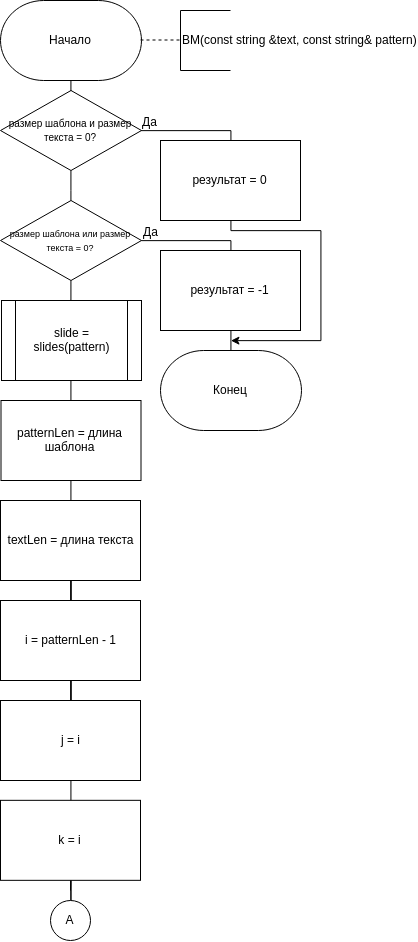
\includegraphics[height=20cm]{BM1}}
\caption{Схема алгоритма Бойера-Мура}
\label{fig:image}
\end{figure}

\begin{figure}[h]
\center{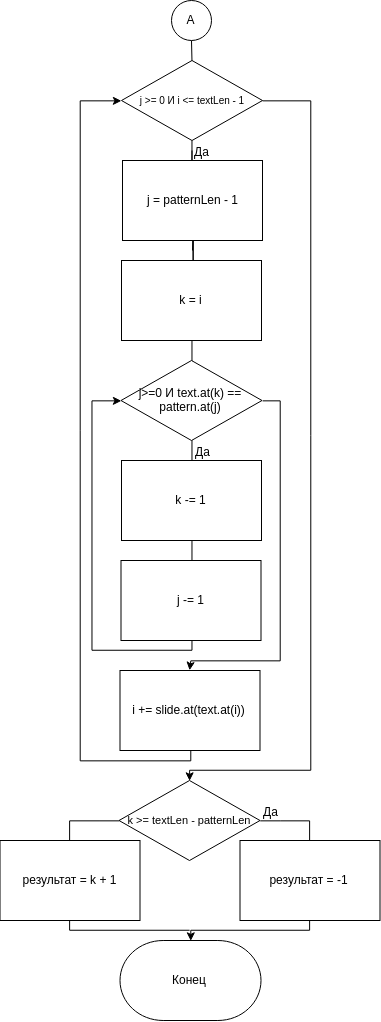
\includegraphics[height=20cm]{BM2}}
\caption{Схема алгоритма Бойера-Мура (продолжение)}
\label{fig:image}
\end{figure}

\begin{figure}[h]
\center{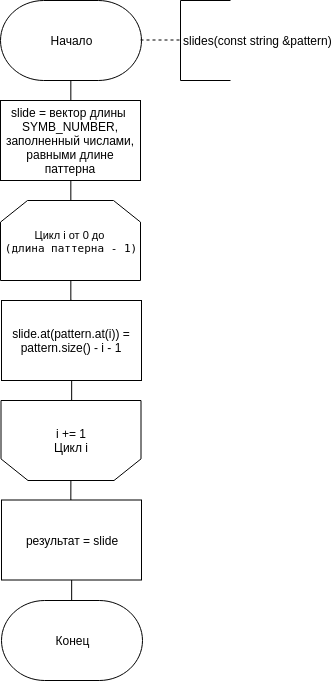
\includegraphics[height=20cm]{slides}}
\caption{Схема метода slides()}
\label{fig:image}
\end{figure}

\begin{figure}[h]
\center{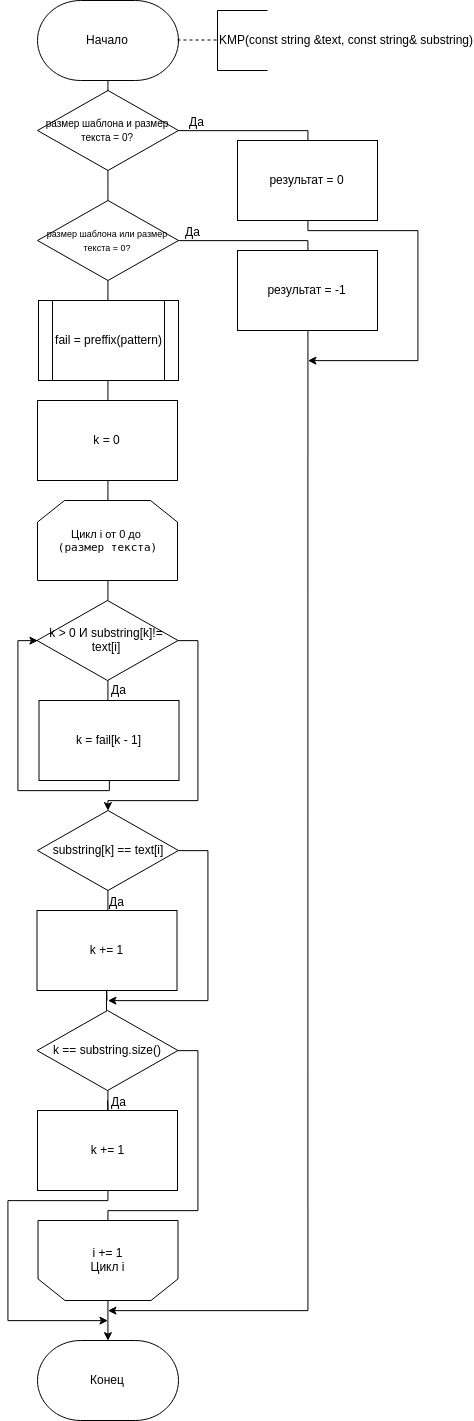
\includegraphics[height=20cm]{KMP}}
\caption{Схема алгоритма Кнута-Морриса-Пратта}
\label{fig:image}
\end{figure}

\begin{figure}[h]
\center{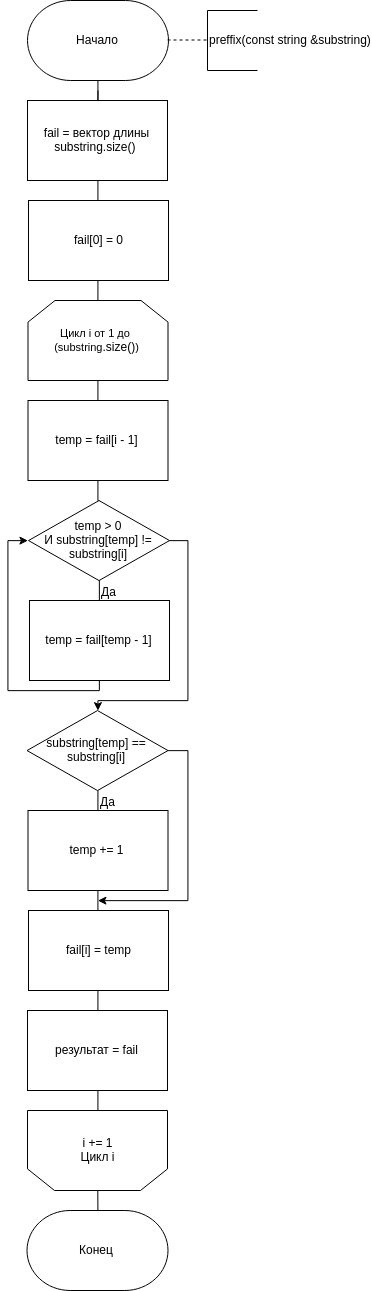
\includegraphics[height=20cm]{preffix}}
\caption{Схема функции preffix()}
\label{fig:image}
\end{figure}


\chapter*{Технологическая часть}
\addcontentsline{toc}{chapter}{Технологическая часть}

В данном разделе будут определены средства реализации и приведен листинг кода.

\section*{Выбор языка программирования}
\addcontentsline{toc}{section}{Выбор языка программирования}

В качестве языка программирования для реализации программы был выбран язык C++ и фреймворк Qt, потому что:
\begin{itemize}
	\item язык C++ имеет высокую вычислительную производительность;
	\item язык C++ поддерживает различные стили программирования;
	\item в Qt существует удобный инструмент для тестирования - QtTest - который позволяет собирать тесты в группы, собирать результаты выполнения тестов, а также уменьшить дублирование кода при схожих объектах тестирования.
\end{itemize}

\section*{Сведения о модулях программы}
\addcontentsline{toc}{section}{Сведения о модулях программы}

Программа состоит из следующих файлов:
\begin{itemize}
	\item main.cpp - главный файл программы;
	\item search.h, search.cpp - файл и заголовочный файл, в котором расположена реализация алгоритма КМП и алгоритма БМ;
	\item testsearch.h, testsearch.cpp - файл и заголовочный файл, в котором расположены тесты.
\end{itemize}

\section*{Листинги кода алгоритмов}
\addcontentsline{toc}{section}{Листинги кода алгоритмов}

В листинге 1 приведена реализация алгоритма Кнута-Морриса-Пратта. В листинге 2 приведена реализация алгоритма Бойера-Мура. В листинге 3 приведена реализация функции slides(), которая используется в алгоритме Бойера-Мура для вычисления сдвигов. В алгоритме Бойера-Мура используется константа, которая равна количеству символов в Ascii-таблице (SYMB\_NUMBER = 128).

\begin{lstlisting}[label=some-code,caption=Агоритм Кнута-Морриса-Пратта]
int KMP(const string &text, const string& substring)
{
    if (text.size() == 0 && substring.size() == 0)
        return 0;
    else if(text.size() == 0 || substring.size() == 0)
        return -1;

    // prefix-function
    vector<size_t> fail(substring.size());
    fail[0] = 0;
    for (unsigned int i = 1; i < substring.size(); ++i)
    {
        size_t temp = fail[i - 1];
        while ((temp > 0) && (substring[temp] != substring[i]))
        {
            temp = fail[temp - 1];
        }
        if (substring[temp] == substring[i])
        {
            ++temp;
        }
        fail[i] = temp;
    }

    // Search
    for (unsigned long k = 0, i = 0; i < text.size(); ++i)
    {
        while ((k  > 0) && (substring[k] != text[i]))
        {
            k = fail[k - 1];
        }
        if (substring[k] == text[i])
        {
            ++k;
        }
        if (k == substring.size())
        {
            return static_cast<int>(i - substring.size() + 1);
        }
    }
    return -1;
}
\end{lstlisting}

\begin{lstlisting}[label=some-code,caption=Агоритм Бойера-Мура]
int BM(const string &text, const string& pattern)
{
    if (text.size() == 0 && pattern.size() == 0)
        return 0;
    else if(text.size() == 0 || pattern.size() == 0)
        return -1;

    vector<size_t> slide = slides(pattern);

    int patternLen = static_cast<int>(pattern.size());
    int textLen = static_cast<int>(text.size());

    int i = patternLen - 1;
    int j = i;
    int k = i;
    while (j >= 0 && i <= textLen - 1)
    {
        j = patternLen - 1;
        k = i;
        while (j >= 0 && text.at(k) == pattern.at(j))
        {
            k--;
            j--;
        }
        i += slide.at(text.at(i));
    }
    if (k >= textLen - patternLen)
    {
        return -1;
    }
    else
    {
        return k + 1;
    }
}
\end{lstlisting}

\begin{lstlisting}[label=some-code,caption=Функция slides()]
vector<size_t> slides(const string &pattern)
{
    vector<size_t> slide(SYMB_NUMBER, pattern.size());
    for (unsigned int i = 0; i < pattern.size() - 1; ++i)
    {
        slide.at(pattern.at(i)) = pattern.size() - i - 1;
    }
    return slide;
}
\end{lstlisting}

\section*{Тесты}
\addcontentsline{toc}{section}{Тесты}

Тестирование проводилось с помощью модуля QtTest. Для этого был написан класс TestSearch. Каждый алгоритм тестировался на заранее заготовленном наборе тестовых данных.
Использованный набор тестовых данных приведен в таблице 1.

Все написанные тесты были пройдены.

\begin{table}[h]
	\caption{Набор тестовых данных}
	%\begin{center}
		\begin{tabular}{| c | c | c |}
	 	\hline
		Текст & Шаблон & Ожидаемый индекс \\ [0.5ex]
	 	\hline\hline
    \grqq there they are \grqq & \grqq they \grqq & 6 \\ \hline
    \grqq there they are \grqq & \grqq there \grqq & 0 \\ \hline
    \grqq there they are \grqq & \grqq are \grqq & 11 \\ \hline
    \grqq there they are \grqq & \grqq hh \grqq & -1 \\ \hline
    \grqq there they are \grqq & \grqq there they are \grqq & 0 \\ \hline
    \grqq \grqq & \grqq dsd \grqq & -1 \\ \hline
    \grqq \grqq & \grqq \grqq & 0 \\ \hline
    \grqq abc \grqq & \grqq \grqq & -1 \\ \hline
    \grqq there they are \grqq & \grqq tt \grqq & -1 \\ \hline
    \grqq there they are \grqq & \grqq ee \grqq & -1 \\ \hline
    \grqq there they are \grqq & \grqq aa \grqq & -1 \\ \hline
	\end{tabular}
%\end{center}
\end{table}

\section*{Примеры работы алгоритмов}
\addcontentsline{toc}{section}{Примеры работы алгоритмов}

Рассмотрим на конкретных примерах работу алгоритма Кнута-Морриса-Пратта и алгоритма Бойера-Мура.

\subsection*{Алгоритм Кнута-Морриса-Пратта}
\addcontentsline{toc}{section}{Алгоритм Кнута-Морриса-Пратта}

Пусть у нас есть алфавит из пяти символов: a, b, c, d, e и мы хотим найти вхождение образца “abbad” в строке “abeccacbadbabbad”.

Таблица преффиксов будет выглядеть так.

\begin{table}[h]
	%\begin{center}
		\begin{tabular}{| c | c | c | c | c |}
	 	\hline
		a & b & b & a & d \\ \hline
    0 & 0 & 0 & 1 & 0 \\ \hline
		\end{tabular}
	%\end{center}
\end{table}

Начало поиска.

\begin{table}[h]
	%\begin{center}
		\begin{tabular}{| c | c | c | c | c | c | c | c | c | c | c | c | c | c | c | c |}
	 	\hline
		a & b & e & c & c & a & c & b & a & d & b & a & b & b & a & d \\ \hline
    a & b & b & a & d & & & & & & & & & & & \\ \hline
		& & a & b & b & a & d & & & & & & & & & \\ \hline
	  & & & a & b & b & a & d & & & & & & & & \\ \hline
		& & & & a & b & b & a & d & & & & & & & \\ \hline
		& & & & & a & b & b & a & d & & & & & & \\ \hline
		& & & & & & a & b & b & a & d & & & & & \\ \hline
		& & & & & & & a & b & b & a & d & & & & \\ \hline
		& & & & & & & & a & b & b & a & d & & & \\ \hline
		& & & & & & & & & a & b & b & a & d & & \\ \hline
		& & & & & & & & & & a & b & b & a & d & \\ \hline
		& & & & & & & & & & & a & b & b & a & d \\ \hline
		\end{tabular}
	%\end{center}
\end{table}

Совпадение найдено.

\begin{table}[h]
	%\begin{center}
		\begin{tabular}{| c | c | c | c | c | c | c | c | c | c | c | c | c | c | c | c |}
	 	\hline
		a & b & e & c & c & a & c & b & a & d & b & a & b & b & a & d \\ \hline
      &   & a & b & b & a & d & & & & & & & & & \\ \hline
		\end{tabular}
	%\end{center}
\end{table}

Конечный автомат представлен на рисунке 6.

\begin{figure}[h]
\center{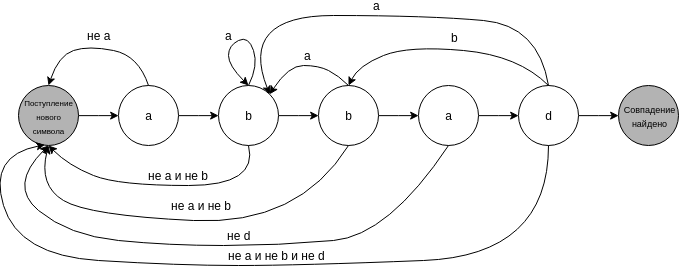
\includegraphics[width=15cm]{kmp_avt}}
\caption{Конечный автомат в алгоритме КМП}
\label{fig:image}
\end{figure}

\subsection*{Алгоритм Бойера-Мура}
\addcontentsline{toc}{section}{Алгоритм Бойера-Мура}

Пусть у нас есть алфавит из пяти символов: a, b, c, d, e и мы хотим найти вхождение образца “abbad” в строке “abeccacbadbabbad”.

Таблица смещений будет выглядеть так.

\begin{table}[h]
	%\begin{center}
		\begin{tabular}{| c | c | c | c | c |}
	 	\hline
		a & b & c & d & e \\ \hline
    1 & 2 & 5 & 5 & 5 \\ \hline
		\end{tabular}
	%\end{center}
\end{table}

Начало поиска.

\begin{table}[!h]
	%\begin{center}
		\begin{tabular}{| c | c | c | c | c | c | c | c | c | c | c | c | c | c | c | c |}
	 	\hline
		a & b & e & c &  \textcolor{red}{c} & a & c & b & a & d & b & a & b & b & a & d \\ \hline
    a & b & b & a &  \textcolor{red}{d} & & & & & & & & & & & \\ \hline
		\end{tabular}
	%\end{center}
\end{table}

Последний символ образца не совпадает с наложенным символом строки. Сдвигаем образец вправо на 5 позиций.
\newpage

\begin{table}[h]
	%\begin{center}
		\begin{tabular}{| c | c | c | c | c | c | c | c | c | c | c | c | c | c | c | c |}
	 	\hline
		a & b & e & c & c & a & \textcolor{red}{c} & \textcolor{green}{b} & \textcolor{green}{a} & \textcolor{green}{d} & b & a & b & b & a & d \\ \hline
     &  &  &  & & a & \textcolor{red}{b} & \textcolor{green}{b} & \textcolor{green}{a} & \textcolor{green}{d} & & & & & & \\ \hline
		\end{tabular}
	%\end{center}
\end{table}

Второй символ не совпадает, сдвигаем на 5 символов вправо.

\begin{table}[h]
	%\begin{center}
		\begin{tabular}{| c | c | c | c | c | c | c | c | c | c | c | c | c | c | c | c |}
	 	\hline
		a & b & e & c & c & a & \textcolor{red}{c} & \textcolor{green}{b} & \textcolor{green}{a} & \textcolor{green}{d} & b & a & b & b & \textcolor{red}{a} & d \\ \hline
     &  &  &  &  &  &  &  &  &  & a & b & b & a & \textcolor{red}{d} & \\ \hline
		\end{tabular}
	%\end{center}
\end{table}

Последний символ не совпадает, сдвигаем на один символ вправо.

\begin{table}[h]
	%\begin{center}
		\begin{tabular}{| c | c | c | c | c | c | c | c | c | c | c | c | c | c | c | c |}
	 	\hline
		a & b & e & c & c & a & c & b & a & d & b & \textcolor{green}{a} & \textcolor{green}{b} & \textcolor{green}{b} & \textcolor{green}{a} & \textcolor{green}{d} \\ \hline
     &  &  &  &  &  &  &  &  &  &  & \textcolor{green}{a} & \textcolor{green}{b} & \textcolor{green}{b} & \textcolor{green}{a} & \textcolor{green}{d} \\ \hline
		\end{tabular}
	%\end{center}
\end{table}

Совпадение найдено.

Конечный автомат представлен на рисунке 7.

\begin{figure}[!h]
\center{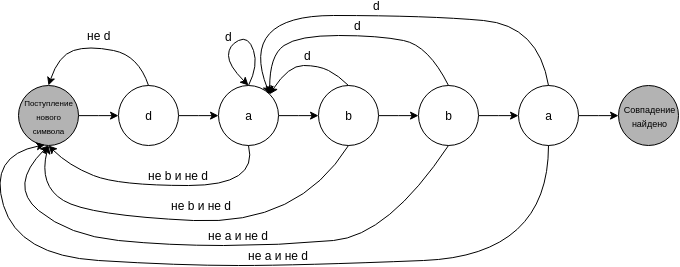
\includegraphics[width=15cm]{bm_avt}}
\caption{Конечный автомат в алгоритме КМП}
\label{fig:image}
\end{figure}

\chapter*{Заключение}
\addcontentsline{toc}{chapter}{Заключение}

Таким образом, в ходе данной лабораторной работы были изучены и реализованы алгоритм Кнута-Морриса-Пратта и алгоритм Бойера-Мура.
Кроме того, была рассмотрена работа этих алгоритмов на конкретных примерах.

\chapter*{Список литературы}
\addcontentsline{toc}{chapter}{Список литературы}

1. Дж. Макконнелл. Основы  современных  алгоритмов. 2-е дополненное  издание. Москва: Техносфера,  2004.  -   368с.

\end{document}
